\documentclass{article}
\usepackage{tikz-feynman}

\begin{document}

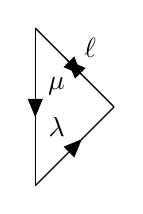
\begin{tikzpicture}
    \begin{feynman}
        \vertex (a) at (0, 1);
        \vertex (b) at (0, -1);
        \vertex (c) at (1, 0);
        \diagram* {
            (a) -- [fermion] (b),
            (a) -- [fermion, edge label=\(\ell\)] (c),
            (b) -- [fermion, edge label=\(\lambda\)] (c),
            (c) -- [fermion, edge label=\(\mu\)] (a)
        };
    \end{feynman}
\end{tikzpicture} = 
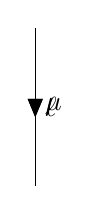
\begin{tikzpicture}
    \begin{feynman}
        \vertex (a) at (0, 1);
        \vertex (b) at (0, -1);
        \diagram* {
            (a) -- [fermion, edge label=\(\ell\)] (b),
            (a) -- [fermion, edge label=\(\mu\)] (b)
        };
    \end{feynman}
\end{tikzpicture}

\end{document}